\documentclass[tikz,border=10pt]{standalone}
\usepackage{tikz}
\usepackage{amsmath}
\usetikzlibrary{arrows.meta, positioning}

\definecolor{susceptible}{RGB}{31,119,180}
\definecolor{exposed}{RGB}{255,127,14}
\definecolor{infectious}{RGB}{44,160,44}
\definecolor{recovered}{RGB}{214,39,40}

\begin{document}
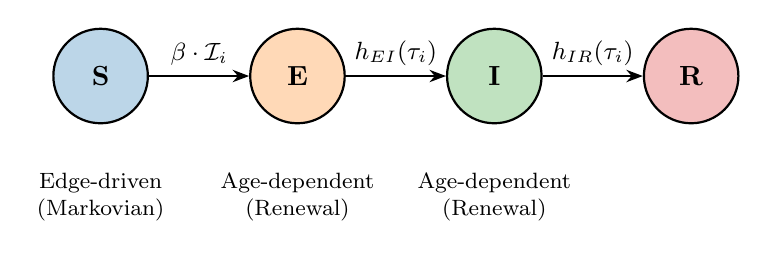
\begin{tikzpicture}[
    state/.style={circle, draw, thick, minimum size=1.2cm, font=\bfseries},
    arrow/.style={-{Stealth[scale=0.9]}, thick},
    label/.style={font=\small, midway}
]

\node[state, fill=susceptible!30] (S) at (0,0) {S};
\node[state, fill=exposed!30] (E) at (2.5,0) {E};
\node[state, fill=infectious!30] (I) at (5,0) {I};
\node[state, fill=recovered!30] (R) at (7.5,0) {R};

\draw[arrow] (S) -- node[above, label] {$\beta \cdot \mathcal{I}_i$} (E);
\draw[arrow] (E) -- node[above, label] {$h_{EI}(\tau_i)$} (I);
\draw[arrow] (I) -- node[above, label] {$h_{IR}(\tau_i)$} (R);

\node[below=0.5cm of S, font=\footnotesize, align=center] {Edge-driven\\(Markovian)};
\node[below=0.5cm of E, font=\footnotesize, align=center] {Age-dependent\\(Renewal)};
\node[below=0.5cm of I, font=\footnotesize, align=center] {Age-dependent\\(Renewal)};

\end{tikzpicture}
\end{document}
